\documentclass{standalone}
\usepackage{pgfplots}
\pgfplotsset{compat=1.7}

\begin{document}
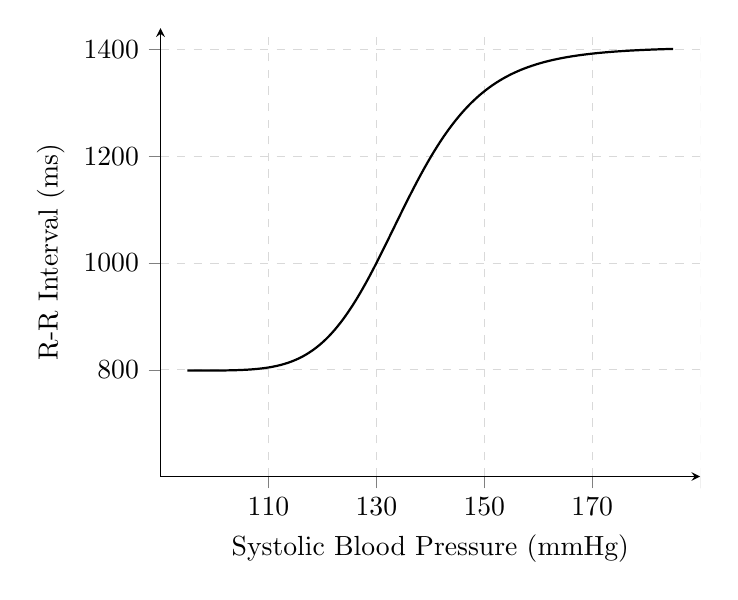
\begin{tikzpicture}


\begin{axis}[
        axis lines=middle,
        grid = major,
        grid style={dashed, gray!30},
	ymin = 0,
	ymax = 210,
	xmin = 0,
	xmax =100,
	 ylabel near ticks,
	xlabel near ticks,
	yticklabels={},
	xticklabels={110,120,110,130,150,170},
yticklabels = {,,800,1000,1200,1400},
        xlabel=Systolic Blood Pressure (mmHg),
        ylabel=R-R Interval (ms),
        tick align=outside,
        enlargelimits=false,
ylabel style={align=center},
legend pos= north west,
legend style={font=\small, cells={align=left}}]

\addplot[domain=5:95, black, thick,samples=500] {201.2206 + (49.62661 - 201.2206)/(1 + (x/48.27129)^5.592923)^1.346863};

\end{axis}

\end{tikzpicture} 
\end{document}